Differential abundance analysis is controversial throughout microbiome research. Current gold standard
approaches require laborious measurements of total biomass to accurately determine taxonomic shifts
among samples. Therefore, most studies rely on making conclusions based off changes in relative abundance.
We highlight commonly made pitfalls in comparing relative abundance across samples and identify two solutions that
reveal microbial changes without the need to estimate total biomass. We define the notion of "reference frames",
which provide deep intuition about the compositional nature of microbiome data. In an oral time series experiment,
reference frames alleviate false positives and produce consistent results on both raw and cell count
normalized data. Furthermore, reference frames identify consistent, differentially abundant
microbes previously undetected in two independent published datasets from subjects with atopic dermatitis.
These methods allow re-assessment of published relative abundance data to reveal reproducible microbial changes
from standard sequencing output without the need for new molecular assays.

\section*{Introduction}
Next-generation sequencing data used to study the microbiome is inherently compositional and routinely provides information in the form of relative abundances, independent of the total biomass of the original sample. Numerous analytical approaches including rarefaction\cite{Weiss2015-gn}, median\cite{Love2014-sn}, and quantile normalization\cite{Love2014-sn,Paulson2013-mm} have been proposed for comparing compositional samples. However, these analytical solutions cannot control false discovery rates\cite{Russel2018-na, Hawinkel2017-ax}, and their application contributes to lack of reproducibility among microbiome studies\cite{Gloor2015-zq}. Here we illustrate mathematical challenges in analyzing compositional microbiome data from DNA sequence reads, and define the concept of “reference frames” for inferring changes in abundance.

\subsection{Why using relative abundance data to evaluate changes in abundance can be misleading}
To illustrate the pitfalls of inferring changes in abundance among samples using relative abundance data, consider the following example (Fig 1). Samples from a population containing only two taxa (orange and blue) are collected pre- and post-treatment. Before treatment, the two taxa occur in equal proportions. After treatment, the orange taxon is twice as abundant as the blue taxon. Did orange increase and blue decrease?

Many different scenarios could actually lead to the same observation. For example, the orange taxon could quadruple and the blue taxon only double. The orange taxon could remain constant, and the blue taxon halve. Or the orange taxon could halve, but the blue taxon could decrease four-fold. Because we only observe relative abundance data, we cannot differentiate among these outcomes, which have markedly different biological significance. Infinite different outcomes produce the same 2:1 ratio of orange to blue, greatly complicating the generation of a meaningful null hypothesis and therefore yielding misleading p-values when the incorrect null hypothesis is chosen.

\begin{figure}
  %%%\includegraphics{something} % this command will be ignored
  \centering
  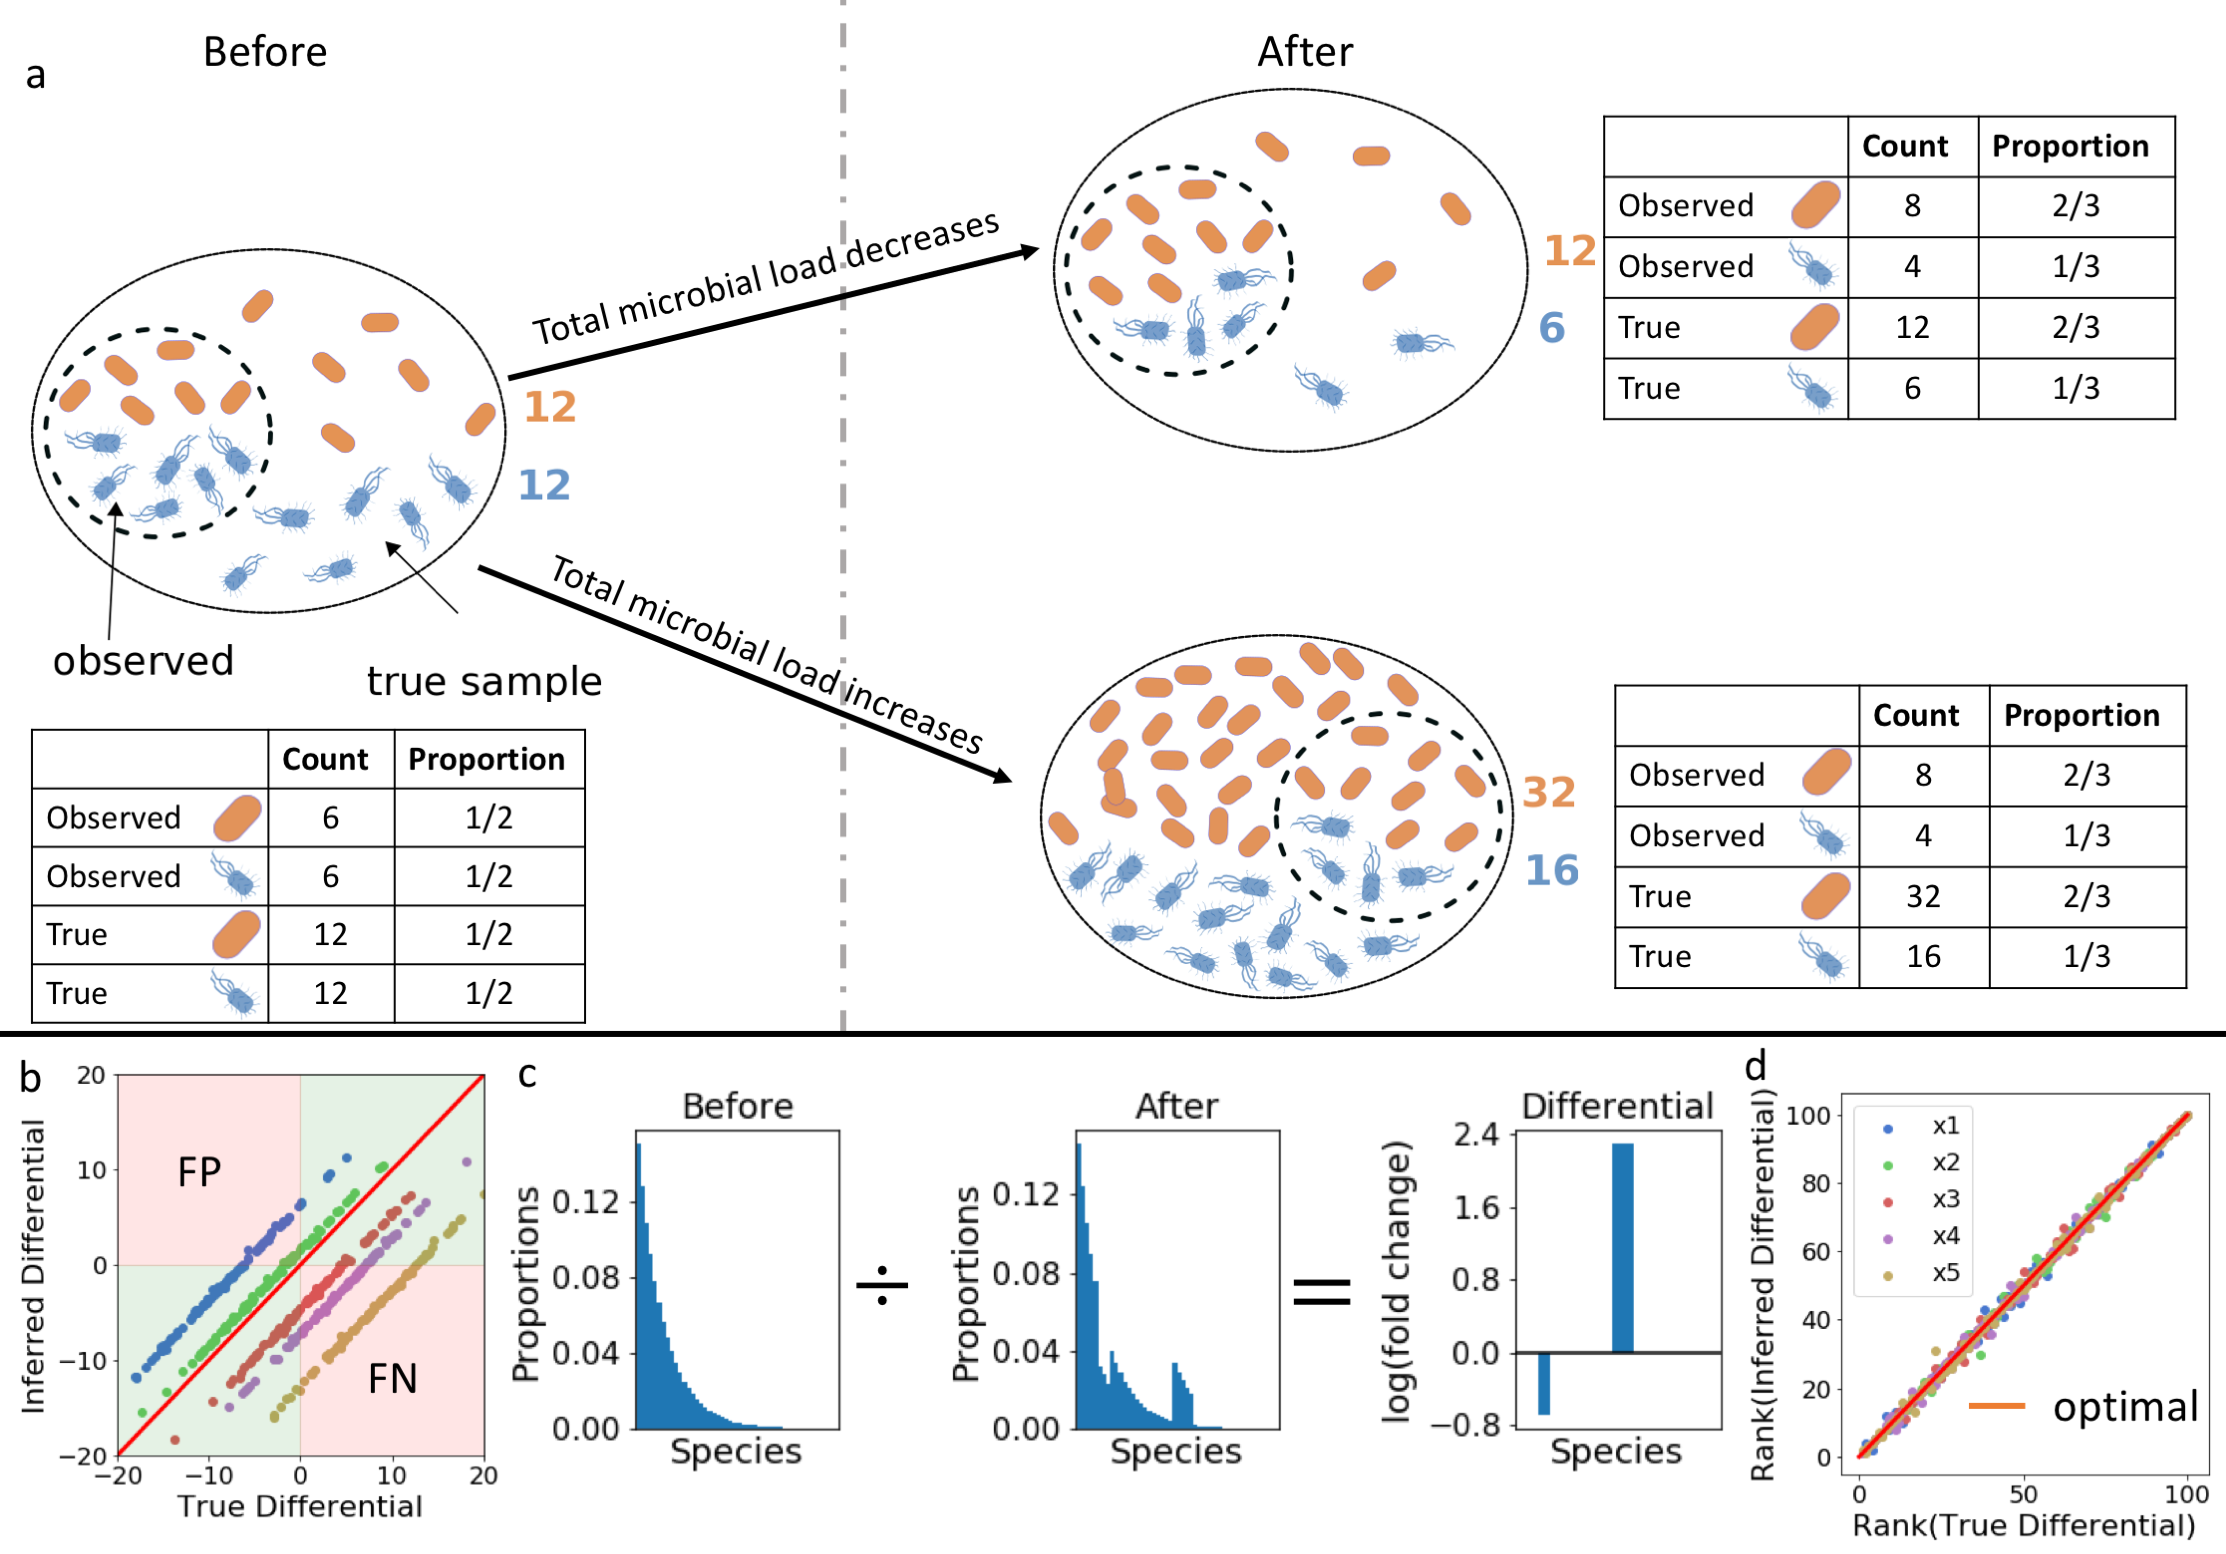
\includegraphics[width=0.8\textwidth]{ch4/Figure1.png}
  \caption[Illustration demonstrating statistical limitations inherent to compositional datasets.]{
    Illustration demonstrating statistical limitations inherent in compositional datasets. (a) Two different biological scenarios can yield the exact same proportions of taxa  in samples from a population pre- and post-treatment. (b) Simulated datasets plotting the true differential obtained using absolute abundance data on the x-axis, versus the inferred differential obtained using relative abundance data on the y-axis. Each dot represents a taxon in the dataset, and the colors represent datasets with various ratios of total microbial load (‘K’) between before and after samples. The red line represents the optimal scenario where the samples have equal microbial load. This illustrates the prevalence of either false positives (\gls{fp}) or false negatives (\gls{fn}) when performing differential abundance analysis on samples with unequal total microbial load. The presence of either (\gls{fp})s or (\gls{fn})s is dictated by a nonlinear function of the true differential (see online methods). (c) An illustration of differential proportions of bacterial species before and after treatment. (d) Same data as (b) but plotting the rank of the differentials, demonstrating that ranks are equivalent regardless of differences in microbial load.}
\end{figure}

\subsection{Microbiome measurement data is inherently compositional}

Multiple processing steps are required to generate microbiome sequencing data. Samples are collected from a much larger population (e.g. fecal material from the gut, or water sample from the ocean). From these samples, a subsample is used for DNA extraction (e.g. a swab from a fecal sample, or an aliquot of a water sample). Another subsample of the extracted DNA is then used as input for PCR, a subset of the resulting amplicon is pooled into a library, and a subset of the library is sequenced.

By the time quality-filtered sequencing data is obtained, the sequences reflect only a small subset of the population and are not an accurate representation of the microbial load in the original sample\cite{Vandeputte2017-jl}. Analyzing purely compositional data (e.g. DNA sequencing data) with conventional statistical tools has led to false discovery rates approaching 100\%\cite{Mandal2015-xw,Morton2017-dz}. Therefore, in addition to compositional data from sequencing, quantitative information about total microbial load is necessary to determine which microbes are changing.

\subsection{Challenges to microbial load quantification}

Multiple approaches at each level of sample processing have been proposed to quantify the total microbial load from environmental samples. Adding a known amount of reference DNA as an internal standard has been used to extrapolate the amount of starting nucleic material\cite{Smets2015-od, Tkacz2018-fp}. Normalization by this method is complicated due to the calibration challenges of choosing the proper amount of internal standard\cite{Tkacz2018-fp,Smets2015-od}. At the extraction level, quantitative PCR (qPCR) of genomic DNA with ‘universal’ primers against the 16S rRNA gene has be deployed to estimate total microbial load\cite{Nadkarni2002-og}. However, it is impossible to prevent primer bias, resulting in uneven amplification of rRNA genes across species. Further, quantification by both spike-in and qPCR is performed on multiple subsets of the original sample.  Quantifying microbial load by flow cytometry is performed on the original sample, and is agnostic to nucleotide sequences. One recent study reported that adding quantitative information obtained by flow cytometry dramatically improved interpretation of 16S rRNA gene amplicon sequencing data\cite{Vandeputte2017-jl}. However, flow cytometry requires expensive equipment, experienced users, and limits throughput.

The total microbial load of an environmental sample is only one dimension of measurement among the hundreds to thousands of dimensions measured by microbial relative abundances. If the abundance of a single taxon and the relative abundance of all taxa is known, it is feasible to compute the absolute abundance of all taxa. As such, considerable information rests in relative abundances, and important insights can be gleaned without costly microbial quantification methods. Below we describe two methods to evaluate relative differential abundance independent of microbial load information.

\subsection{Using ratios circumvents bias without microbial load quantification}
Computing changes in abundance from compositional data introduces a bias due to the lack of total microbial load (Fi 1. approach\#1). Simulated data in Fig 1b shows how different biases (i.e. ratios between total microbial loads) can cause either false positives or false negatives.
By simply comparing the ratio of taxa between samples, the bias constant introduced by unknown microbial load cancels out. For instance, if an observed taxon X changes from 10\% to 20\% in relative abundance, that observation can be irreproducible across studies or samples because of fluctuations in abundance of other taxa. Changes in the abundance of taxon X relative to taxon Y should be consistent. Taking the logarithm of this ratio (log-ratio) enforces symmetry around zero, giving equal weight to relative increases and relative decreases.

\subsection{A novel approach to rank differential abundance}
Comparing ratios of taxa can circumvent the bias introduced by unknown microbial loads. However, choosing taxa for comparison from the thousands in a given sample set can be challenging. By ranking the log-ratio abundance changes of each taxon (what we refer to as “differentials”), an accurate depiction of compositional change in a dataset can be obtained and taxa can be prioritized (Fig 1c). As shown in Fig 1d, the rank of each taxon’s differential is independent of the changes in the absolute microbial load, yielding an identical ranking of microbial differences between the relative and absolute abundances. However, because of the unknown bias described above, we cannot infer based on rank alone if a microbe has changed, and therefore a coefficient of zero does not imply that the microbe has not changed abundance.

Differentials can be estimated directly using explicit count-based regression models (see online methods). For example, multiple studies have shown that multinomial linear models can infer differentials without adding pseudocounts to handle sampling zeros\cite{Silverman2018-ql,Aijo2018-jp, Grantham2017-gv,Xia2013-nd}. The coefficients from multinomial regression analysis can be interpreted as feature importances or rankings commonly employed by machine learning methods, and can be ranked to determine which taxa are changing the most between samples. We refer to this ranking procedure as differential ranking (DR).

\subsection{Reference frames enable reproducible compositional data comparisons}
We argue that analyzing compositional data requires a choice of “reference frames” for inferring changes in abundance. By "reference frame", we draw on the concept from physics where velocity is measured "relative to" another moving object. As microbial populations change, we can constrain our inferences to how microbial populations change relative to reference frames given by other microbial populations. The choice of numerator and denominator in a log-ratio determines the reference frame for inferring changes. In DR, the differential abundances of each taxon serve as a reference to each other when they are ranked numerically. To demonstrate these principles, we confirm the robustness of these two methods of employing reference frames in real life datasets.

\subsection{Value of reference frames in the analysis of microbes in unstimulated saliva}
We demonstrate the utility of DR in a sample set with dramatic differences in total microbial load. Unstimulated saliva samples were collected from 8 individuals before and after brushing their teeth (morning and night, n=32), and processed in parallel for microbial load quantification with flow cytometry and 16S rRNA gene amplicon sequencing. Importantly, participants were asked to provide unstimulated saliva for exactly 5 minutes, so in addition to estimating microbial concentration, we could obtain a proxy for the total microbial load taking into account salivary flow rate. As expected, the total microbial load significantly decreased after brushing teeth (Fig. 2a).

\begin{figure}
  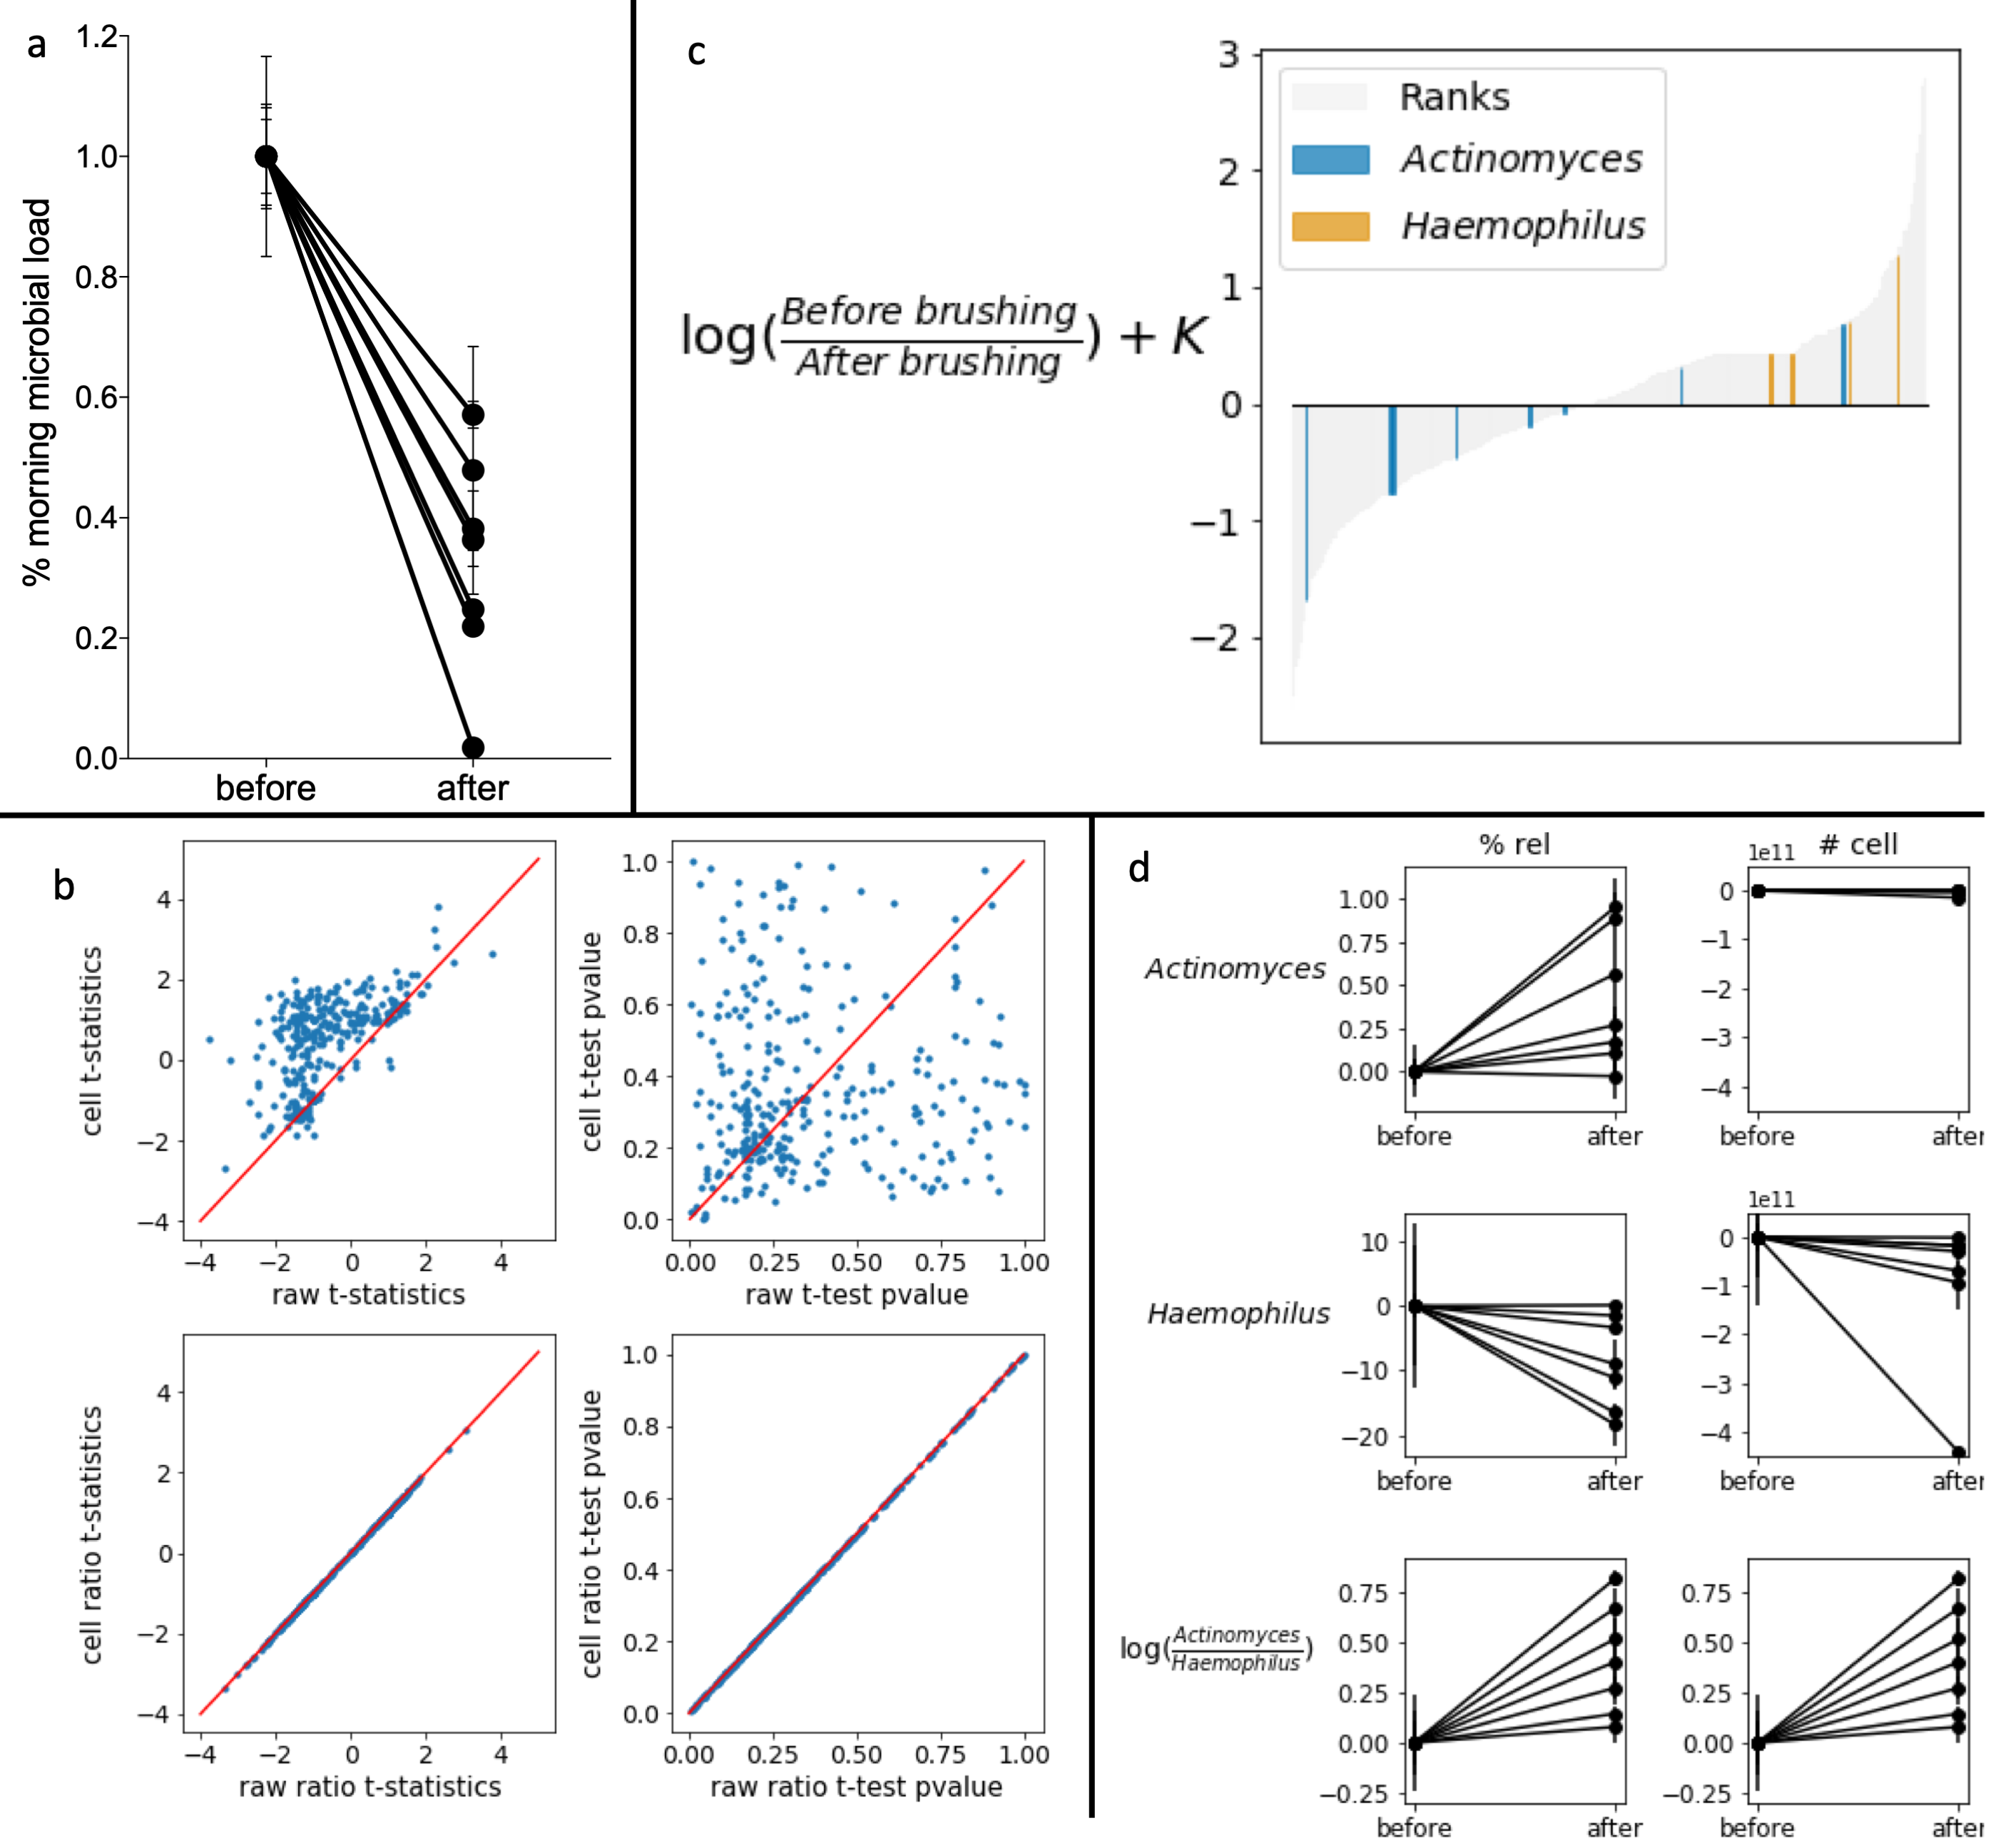
\includegraphics[width=1\textwidth]{ch4/Figure2.png}
  \caption[Analysis of salivary microbiota before and after brushing teeth.]{
    Analysis of salivary microbiota before and after brushing teeth. (a) Flow cytometry-quantified microbial
    load in unstimulated saliva collected for 5 minutes normalized to before brushing teeth. Each line corresponds
    to a different volunteer. (b) A comparison of t-statistics (left) and p-values (right) on individual taxa (top)
    and ratio between each taxa to \textit{Actinomyces} (bottom) between relative abundance data (x-axis) and cell
    count-normalized data (y-axis). (c) Microbial ranks estimated from multinomial regression applied to oral time
    series dataset with \textit{Actinomyces} and \textit{Haemophilus} highlighted.  The y-axis represents the log-fold change that is
    known up to some bias constant K, and the x-axis numerically orders the ranks of each taxa in the analysis
    (d) A comparison of relative abundance vs cell counts of \textit{Actinomyces}, \textit{Haemophilus} and log(\textit{Actinomyces}:\textit{Haemophilus})
    before and after brushing teeth. Only the differences since the before time point are visualized.}
\end{figure}

For both relative and cell count-normalized data, we performed paired t-tests to evaluate the change in abundance of each taxon before and after brushing teeth (Fig. 2b). Applying t-tests to the relative data had a high false-positive rate, as seen by the disagreements between the cell count-normalized and relative t-statistics (Spearman r=$0.53$). Further, there was absolutely no correlation in p-value distribution between the relative and cell count-normalized data (Spearman r=$0.09$), highlighting the fallacy in calculating a p-value without a valid null hypothesis.

Alternatively, evaluating the ratio between \textit{Actinomyces} and the remaining taxa produced identical t-statistics and p-values between the relative and cell count-normalized data (Spearman r=$1.0$). Ratio-based analyses are unaffected by microbial load (see Methods, equation 3) and result in identical interpretations as one obtains from costly and rate-limiting flow-cytometry measurements.

From the DR analysis (Fig. 2c), we can identify which taxa are changing the most (highest and lowest log-fold change). Here, we highlight \textit{Actinomyces} and \textit{Haemophilus} species, which have very different ranks: \textit{Actinomyces} have low ranks and \textit{Haemophilus} have high ranks. The difference in ranks between these taxa correctly suggests that \textit{Haemophilus} taxa are more prevalent relative to other taxa before brushing, and \textit{Actinomyces} taxa are more prevalent relative to other taxa after brushing. When inspecting t-test results on individual taxon in the relative data, it appears that \textit{Actinomyces} significantly increased (t-statistic=$2.89$, p-value=$0.013$) after brushing teeth and that \textit{Haemophilus} significantly decreased (t-statistic=$-2.593$, p-value=$0.023$). However, cell count data revealed that only \textit{Haemophilus} significantly decreased (t-statistic=$-2.477$, p-value=$0.029$) (Fig. 2d).

The log-ratio of \textit{Actinomyces} and \textit{Haemophilus} between the relative and the cell count-normalized data is identical. While we cannot observe the decrease of \textit{Haemophilus} or the consistency of \textit{Actinomyces} abundance, with the log-ratio of their relative abundance, we can observe the interaction between these two taxa and the increase of \textit{Actinomyces} relative to \textit{Haemophilus} after brushing teeth (t-statistic=$2.833$, p-value=$0.015$)
These results are consistent with our knowledge about oral biogeography. \textit{Haemophilus} is typically found on the periphery of oral biofilms and was likely removed from the biofilm during the brushing process, whereas \textit{Actinomyces} is generally found on the surface of the tooth and acts as an anchor for biofilm attachment\cite{Welch2016-lw}. Importantly, this experiment demonstrates the potential fallibility of relying on relative abundance; It is illogical to conclude that \textit{Actinomyces} increases after tooth brushing despite the increase in relative abundance. As demonstrated by flow cytometry, total microbial load decreases, and while both \textit{Haemophilus} and \textit{Actinomyces} decrease, \textit{Haemophilus} decreases more.

Next, we demonstrate the utility of log-ratios and DR to identify consistent microbial changes across previously published datasets where quantification of microbial load is unavailable.

\subsection{Discovery of interkingdom relationships in atopic dermatitis using reference frames}
The tooth brushing example provides ground truth for using log-ratios and DR, but many clinically relevant microbiome questions involve less obvious differences. Using data from patients with atopic dermatitis (AD), an important skin disease, we demonstrate how viewing relative abundances alone can produce false negatives.

AD has a complex etiology. Many microbiome studies performed using next-generation sequencing have focused on bacterial changes associated with AD, especially the pathogen \textit{Staphylococcus aureus}. The yeast genus \textit{Malassezia} has also been implicated in AD, although conflicting results have been published as to which \textit{Malassezia} species are involved and whether they are more or less prevalent in AD\cite{Glatz2015-ag}. A recent shotgun metagenomic study examined the skin microbiome over time during an AD flare and recovery. The authors observed a decrease in \textit{Staphylococcus aureus} relative abundance in the healthy, recovered skin (non-lesioned) compared to AD flare (lesion), but no significant changes in the relative abundance of \textit{Malassezia} species over time in these AD patients\cite{Byrd2017-eb}.

\begin{figure}
  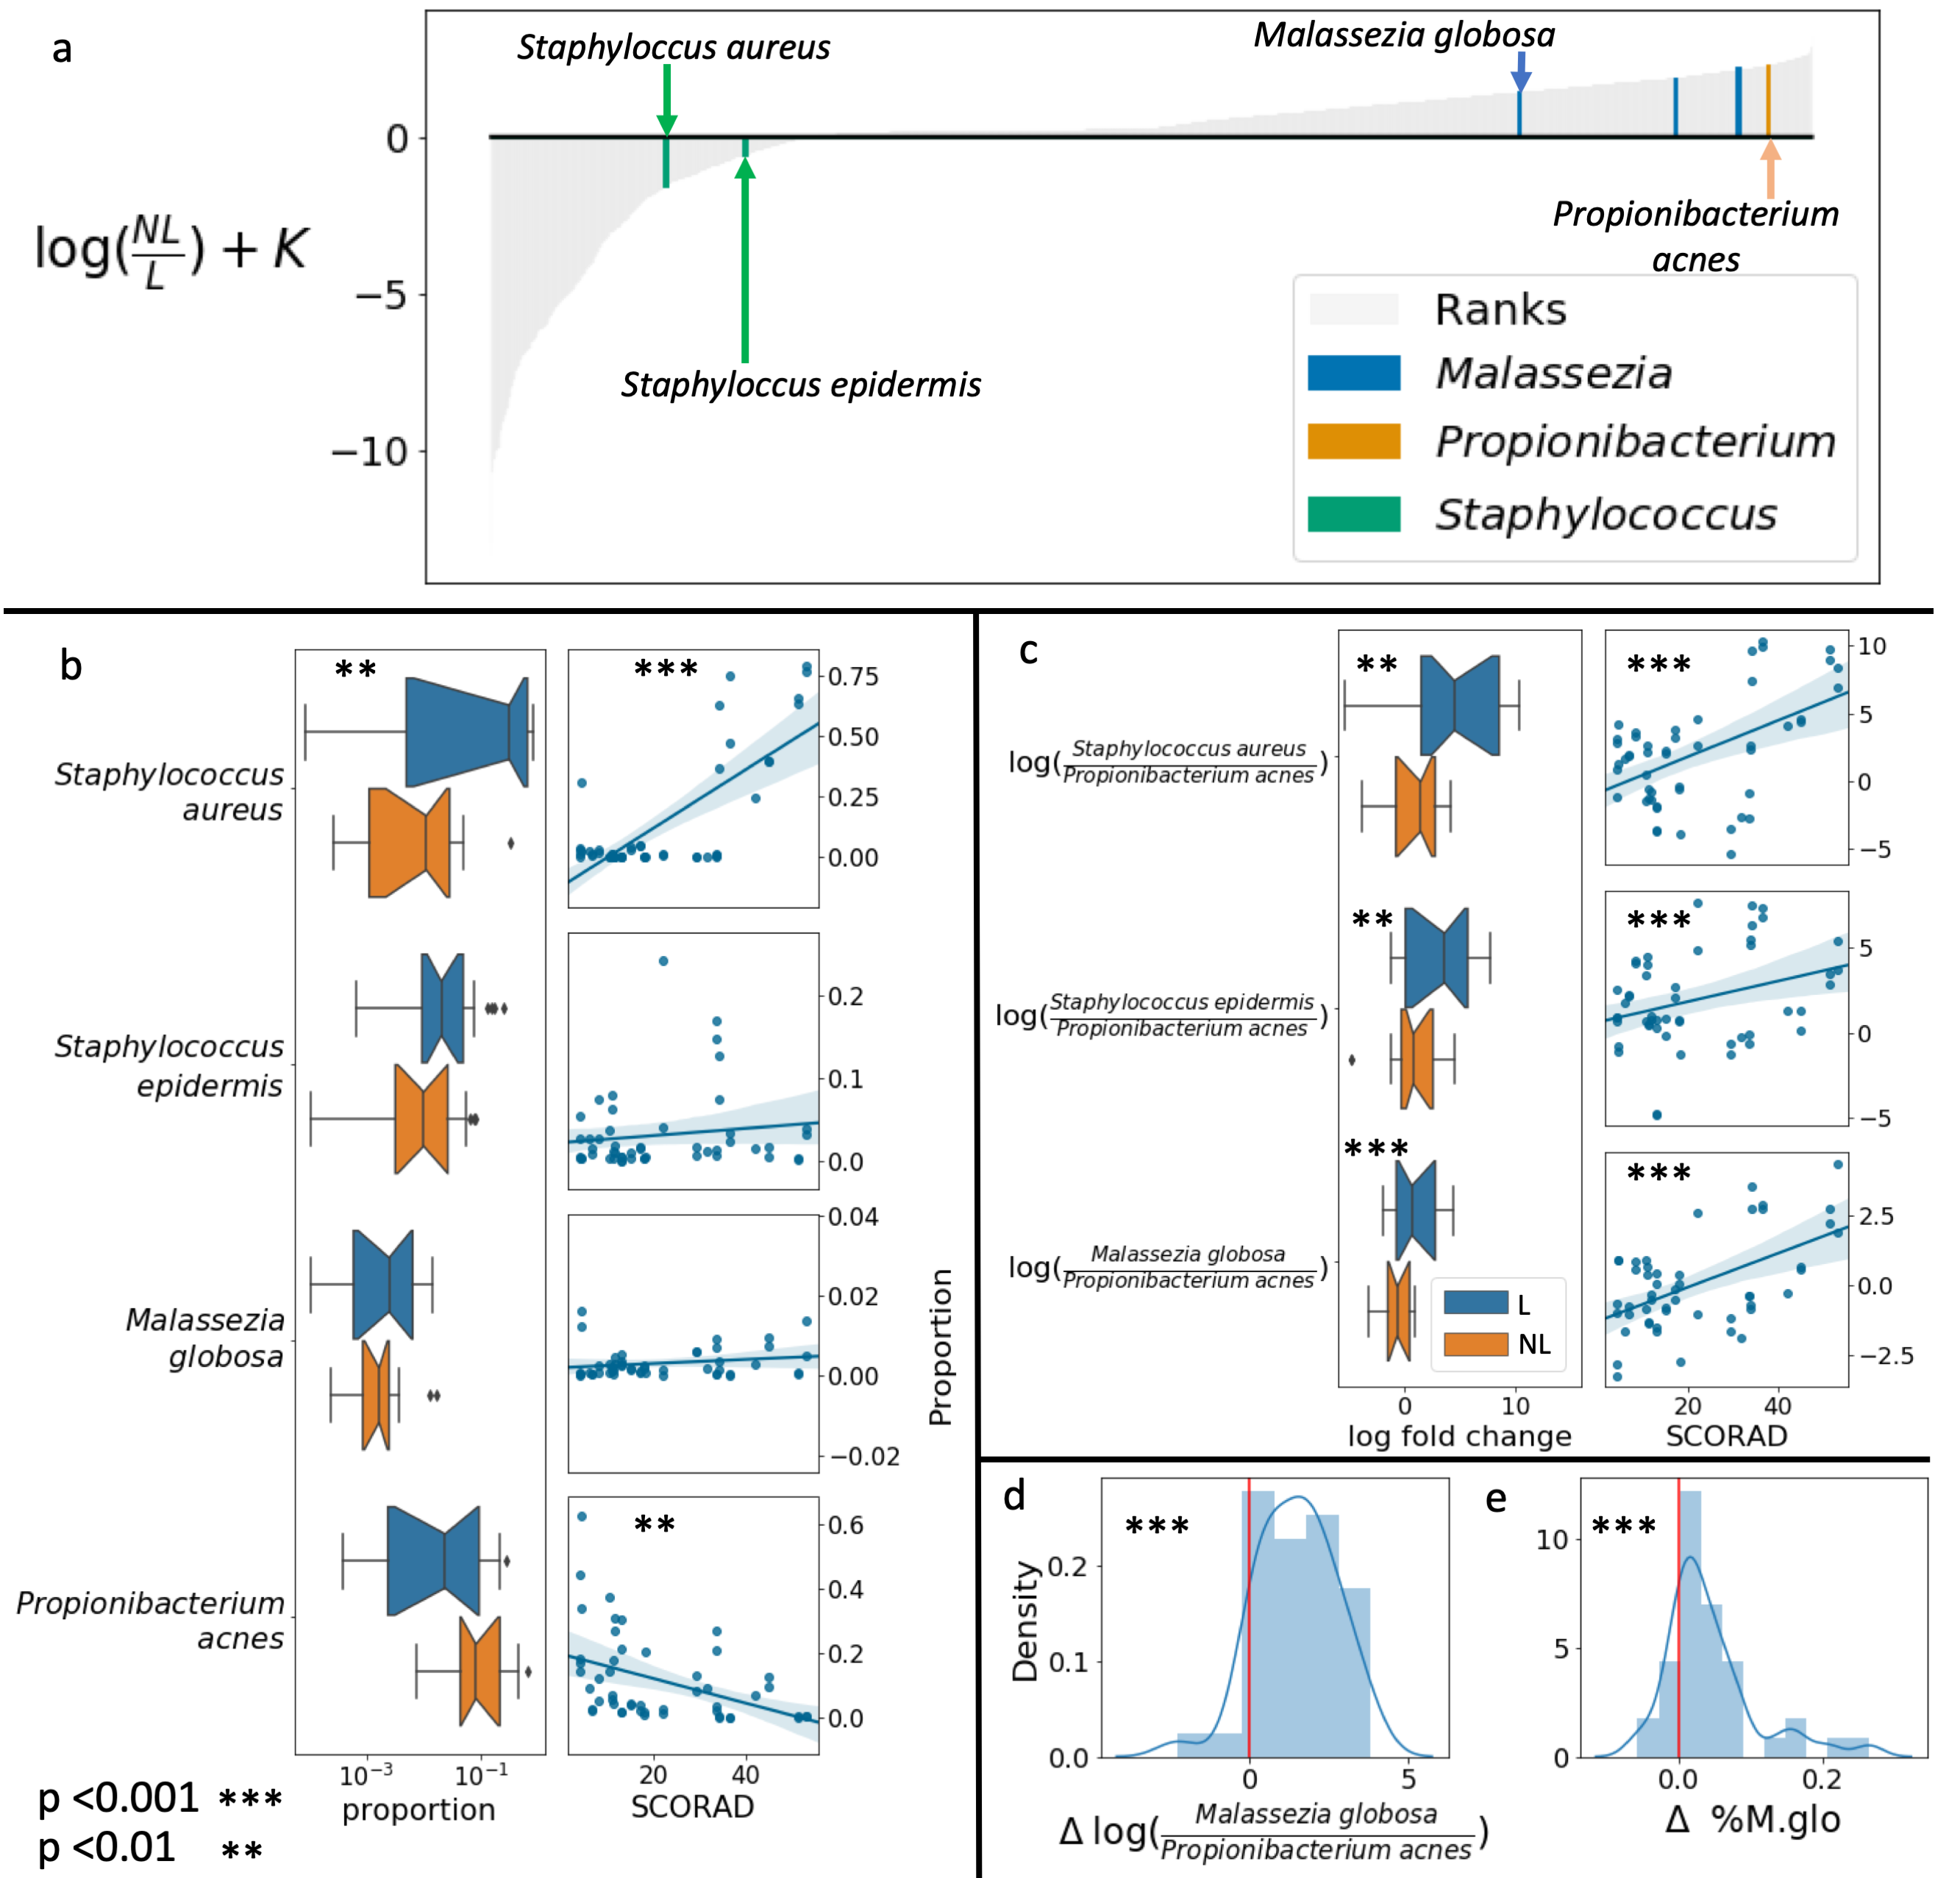
\includegraphics[width=1\textwidth]{ch4/Figure3.png}
  \caption[Comparison of lesioned versus non-lesioned skin in two atopic dermatitis studies.]{
    Comparison of lesioned (L) versus non-lesioned (NL) skin in two atopic dermatitis studies;
    Byrd et al.\cite{Byrd2017-eb}, (a-c) and Leung et al.\cite{Leung-DYM}, (d-e). (a) Microbial ranks estimated from
    multinomial regression applied to shotgun metagenomics from Byrd et al\cite{Byrd2017-eb} with key
    genera highlighted. The y-axis represents the log-fold change that is known up to some bias constant K.
    (b) Proportions of \textit{S. aureus}, \textit{S. epidermidis}, \textit{M. globosa}, and \textit{P. acnes}
    in lesioned (blue) and non-lesioned (orange) skin (left) and correlation of relative abundance
    with \gls{scorad} score (right) (c) Log-ratios of \textit{S. aureus} : \textit{P. acnes} , \textit{S. epidermidis} : \textit{P. acnes} ,
    and \textit{M. globosa} : \textit{P. acnes} (left) and correlation of ratio with \gls{scorad} score.
    (d) Change in log ratio of \textit{M. globosa} : \textit{P. acnes}. (e) Change in
    relative abundance of M. globosa between lesioned and non-lesioned skin from (Leung et al.\cite{Leung-DYM}).}
\end{figure}

Applying compositionally coherent methods to this dataset revealed new insights. Observing the DR results (Fig. 3a), it is apparent that, compared to lesioned skin, \textit{S. aureus} is one of the taxa to decrease the most relative to all other microbes in the non-lesioned sites, followed by \textit{S. epidermidis}, and \textit{M. globosa}. Consistent with the analysis of relative abundance in Fig. 3b, the ratio of \textit{S. aureus : P. acnes} was significantly increased in flare (t-statistic=$2.973$, p-value=$7.811\times 10^{-3}$) and correlated with SCORAD score, a clinical assessment of AD severity (Pearson=$0.747$, p-value=$3.516\times 10^{-6}$). Contrary to previous findings, both \textit{S. epidermidis : P. acnes} and \textit{M. globosa : P. acnes} were also significantly increased in lesioned skin (t-statistic=3.197, p-value=$4.748\times 10^{-3}$, and t-statistic=$4.030$, p-value=$7.16\times 10^{-4}$, respectively) and correlated with SCORAD score (Pearson r=$0.464$, p-value=$6.975 \times 10^{-4}$, and Pearson r=$0.668$, p-value=$1.125\times 10^{-7}$, respectively) (Fig. 3c).

To validate this observation, we analyzed shotgun data from an independent AD dataset\cite{Leung-DYM}.  In this dataset, the relative abundance of \textit{M. globosa} significantly increased between lesioned and non-lesioned skin (Fig. 3e, t-statistic=4.135, p-value=0.0001). But the ratio of \textit{M. globosa : P. acnes} increased even more dramatically in lesioned skin (Fig. 3d, t-statistic=$5.79$, p-value=$8.6 \times 10^{-7}$) (Fig. 3d). These results are congruent with a previous report that \textit{M. globosa} was cultivated more successfully from lesioned versus non-lesioned sites in AD\cite{Falk2005-we}. Thus, DR analysis can identify novel, clinically significant microbial changes which can be validated across cohorts by choosing insightful reference frames.

\section*{Discussion}
Adding information about absolute microbial load between samples can highlight issues inherent in compositional data analysis. However, there are multiple practical and technical challenges in quantifying microbial load. For example, skin swabs are often difficult to use in flow cytometry due to very low biomass and difficulty in transferring intact cells from swabs into liquid solution. Furthermore, skin samples are notoriously sensitive to 16S rRNA gene primer choice making qPCR quantification challenging\cite{Meisel2016-mp}. Similarly, for historically collected samples that exist only as DNA in a freezer or as sequences in a database, flow cytometry approaches to determine absolute microbial load are not feasible.

However, absolute abundances of a community are only one dimension of measurement, and robust, alternative techniques eliminate the need to estimate total biomass. We have demonstrated the validity of using microbial ratios and differential rankings to determine significant changes in microbiome studies by comparing compositional inferences with absolute abundance inferences.

By using flow cytometry to quantify total microbial load, we validated these analytical tools in 16S rRNA gene amplicon sequencing data from unstimulated saliva. We found evidence of false positives when looking exclusively at changes in relative abundance before and after brushing teeth. By evaluating the ratio of \textit{Actinomyces : Haemophilus}, we reached an identical conclusion to our cell-count normalized data without the need for microbial load quantification. The consistency of our results rests in the use of ratios defining reference frames for inferring compositional changes.

Furthermore, we highlighted an example of a false negative in previously generated shotgun metagenomic data from the skin of individuals with AD. We were able to reproduce the findings that \textit{S. aureus}, and to a lesser extent \textit{S. epidermidis}, are differentially abundant in AD lesions. Additionally, using log-ratios and differential ranking, we were also able to show a more subtle but statistically significant change in \textit{M. globosa} abundance in AD lesions. This same result was obtained in two independent metagenomic studies of AD patients and agrees with previous cultivation-based work quantifying increased colony forming units of \textit{M. globosa} in AD lesions.

Consistency between inferences made based on relative and cell count-normalized data is crucial, because in many circumstances it is not possible or practical to estimate total microbial load. The seeming contradiction between microbial load-corrected abundances and relative abundances does not invalidate data from the existing 100,000+ experiments utilizing 16S rRNA gene amplicon or metagenomic sequencing\cite{Shi2018-xe,Gonzalez2018-rv}. Importantly, these techniques are not limited to next generation microbiome sequencing, but can be applied to any experiments involving compositional data (e.g. metabolomics, proteomics, etc.).

Multiple tools have already been developed that can facilitate analysis using log-ratios. For instance, tools such as PhILR, Phylofactoriation and Gneiss provide different means to compute reference frames for log-ratio analysis. However, these methods rely heavily on pseudocounts, because the logarithm of zero is undefined. This can add a substantial amount of bias, especially in sparse datasets. The Differential ranking (DR) procedure circumvents this problem through the use of the multinomial regression.

While various methods of multinomial-based models have been developed\cite{Silverman2018-ql,Aijo2018-jp, Grantham2017-gv,Xia2013-nd}, the interpretation of the resulting model coefficients is usually incorrect. A zero valued coefficient does not imply that the corresponding species abundance hasn’t changed, due to the total biomass bias as discussed in Fig 1. DR provides a novel means to correctly interpret the coefficients of these models. By ranking the coefficients we can determine which taxa have changed the most relative to each other. This subtle distinction acknowledges the limits of analysis of compositional data, and as demonstrated above can have dramatic impacts on data interpretation.

While there are widespread misconceptions concerning how to interpret microbial abundances, there is still much hope for resolving these outstanding controversies. Ongoing efforts at the NIH and EMBL-EBI have already stored petabytes of multi-omics datasets ready to be re-analyzed, and databases, such as Qiita and gcMeta, contain curated data and metadata from hundreds of thousands of samples\cite{Gonzalez2018-rv, Shi2018-xe}. There is much promise for resolving outstanding controversies by re-analyzing these datasets using reference frames to make stable inferences of compositional change.

%
%
\section{Methods}
  If we wanted to compute the change between two samples containing compositions (e.g. relative abundance of microbes) $\bm A=(a_1,...,a_D)$ and $\bm B=(b_1,...,b_D)$ , it would look like
  \begin{align}
    \frac{\bm{A}}{\bm{B}}=\big(\frac{a_1}{b_1} ,\ldots  \frac{a_D}{b_D}\big)
  \end{align}
  If we are only able to measure relative abundances, as is the case with next generation amplicon sequencing, we can only estimate the proportion $p_{a_i}$ for species $i$ in the sample $A$  i.e. $p_{a_i}=\frac{a_i}{N_a}$.  Estimating the true abundance can be done via $a_1=N_a p_{a_1}$, where $N_a$ is the total abundance of sample $A$.  To we wanted to estimate the true change, that can be done as follows
  \begin{align}
    \frac{\bm{A}}{\bm{B}} =
    \frac{N_a \times p_{a_1}}{N_b \times p_{b_1}}, \ldots \frac{N_A \times p_{a_D}}{N_B \times p_{b_D}} =
    \frac{\bm{p_A}}{\bm{p_B}} \times  \frac{N_A}{N_B}
  \end{align}
  To determine if species $i$ abundance has changed between samples $A$ and $B$, we test to see if $\frac{a_i}{b_i}=1$. However as shown above, we cannot perform this test, since the results of this test would be confounded by the total biomass bias $\frac{N_A}{N_B}$.

In many cases, the total biomass cannot be estimated, so any techniques to identify important species will need to alleviate this bias. One alternative is to use ratios. If we choose species D to be the reference species, it is clear that the total biomass cancels as follows
  \begin{align}
    \frac{a_1/a_D}{b_1/b_D}  =  \frac{p_{a_1}/p_{a_D} }{p_{b_1}/p_{b_D}}
  \end{align}
  Another alternative is to use ranks. Since the bias is applied uniformly across the differential, it will not affect the ordering of the species. Hence, ranks are agnostic to the total biomass bias.
  \begin{align}
    rank (\frac{\bm{A}}{\bm{B}}) =
    rank(\frac{\bm{p_A}}{\bm{p_B}} \times \frac{N_A}{N_B}) =
    rank(\frac{\bm{p_A}}{\bm{p_B}} )
  \end{align}

This differential is also commonly referred to as a perturbation in the context of the compositional literature\cite{Pawlowsky-Glahn2015-qb}.
It is important to note that this does not justify using Spearman correlation or other non-parameteric tests such as Kruskal-Wallis applied to relative abundance data since these tests do not satisfy scale invariance\cite{Friedman2012-cn,Lovell_David_Muller_Warren_Taylor_Jennifer_Zwart_Alec_Helliwell2010-na}.

Both of the log-ratios and the differential ranking techniques satisfy scale invariance, meaning that both of these techniques are agnostic to the total biomass.  This concept is critical when analyzing relative abundance data, since this is one step closer to maintaining consistent conclusions between the original environment and the observed sequences.

Estimating log-fold differential expression from relative abundances can result in either false positives (FP) or false negatives (FN) depending on the distribution of true differential expression. Whether FNs or FPs are observed depends on a nonlinear relationship involving the true (unobserved) differential expression. For a p-vector $x$ let us define $LSE(x) = \log(e^{x_1}+ \ldots +e^{x_p})$. If $\bm{\delta}=(\delta_1, \ldots ,\delta_D)$ denotes the true differential expression of the $D$ species between two conditions, let $\bm{\alpha}=LSE(\bm{\delta})$. Further, let $\hat{\bm{\delta}}=(\hat{\delta_1}, \ldots, \hat{\delta_D})$ represent the inferred differential expression from proportional data and $\bm{\hat{\alpha}}=LSE(\bm{\hat{\delta}})$. If $LSE(\delta) > LSE(\hat{\delta})$ then FPs will be observed. In contrast if $LSE(\delta) < LSE(\hat{\delta})$ then FNs will be observed.

\subsection{Multinomial regression}
To perform the differential ranking (DR) analysis, we used multinomial regression. Multinomial regression and related count regression models are commonly used in the context of microbiome analysis. Here, we use the multinomial regression model since these models can reliably estimate the means and can be easily reinterpreted in the context of compositional data analysis.

Counts from the multinomial regression can be formulated in the following generative model
\begin{align*}
  \beta_{jk} &\sim \mathcal{N}(0, \mu_{\beta})\\
  \boldsymbol{\eta_i} &= alr^{-1}(\boldsymbol{X_i} \boldsymbol{\beta})\\
  \boldsymbol{Y_i} &\sim Multinomial(\boldsymbol{\eta_i}) \mbox{ ,}
\end{align*}
where $\boldsymbol{\beta}$ represents the coefficients of the model across all measured covariates $k$. $\boldsymbol{X_i}$ represents the metadata covariates for sample $i$. $\boldsymbol{Y_i}$ represents the measure microbial counts for sample $i$. A normal prior centered around zero was placed on the covariates $\boldsymbol{\beta}$ to serve as regularization to combat issues associated with high dimensionality.

The inverse alr function is a function commonly used in the context of compositional data, give as follows
\begin{align*}
  alr^{-1}(x) &= C[\exp(0, x_1, \ldots, x_{D-1})] & C[x] &= \bigg[ \frac{x_1}{\sum\limits_{i=1}^D x_i}, \ldots, \frac{x_D}{\sum\limits_{i=1}^D x_i} \bigg] \mbox{ .}
\end{align*}
This is also referred to as a degenerate softmax function, which is commonly used in the context of neural networks.  This function is also isomorphic between $\mathbb{R}^{D-1}$ and $\mathcal{S}^D$ (the space of proportions), so this will ward against identifiability issues when estimating these model parameters. The models were estimated using a maximum a posteriori priori (MAP) estimation using stochastic gradient descent.

If we examine the model parameters $\boldsymbol{\beta_k} \in \mathbb{R}^{D-1}$, we reinterpret the quantities given by $alr^{-1}(\boldsymbol{\beta_{k}})$ as differentials as discussed in Fig 1.

It is also worthwhile to note the connection between $\boldsymbol{\beta_k}$ and balances. Since $\boldsymbol{\beta_k}$ is expressed in alr coordinates, there is also a direct connection to ilr coordinates, meaning that $\boldsymbol{\beta_k}$ can also be transformed into balances. More explicitly, the ilr coordinates of these coefficients can be computed as follows
\begin{align*}
  \boldsymbol{\beta_k}^{(ilr)} = ilr_{\boldsymbol{\Psi}}(alr^{-1}(\boldsymbol{\beta_k})) \mbox{ .}
\end{align*}
The resulting coefficients are represented as coordinates given by the orthonormal basis $\boldsymbol{\Psi}$. An example of such a basis can be dervied from bifurcating trees discussed in Morton et al\cite{Morton2017-dz}, Silverman et al\cite{Silverman2016-he} and Washburne et al\cite{Washburne2017-up}. This can allow for relative changes in abundances as given by $alr^{-1}(\boldsymbol{\beta_k})$ to inform which balances are changing in ancestral states given by the tree . The multinomial regression serves as an alternative means to compute regression coefficients discussed in PhILR, Phylofactor and Gneiss, while avoiding issues with imputation and zeros.

The multinomial regression was implemented using Tensorflow\cite{abadi2016tensorflow} and can be found in \\
https://github.com/mortonjt/songbird.

\subsection{Saliva sample collection}
Eight volunteers provided unstimulated saliva so that salivary flow rate could be measured according to a standardized protocol \cite{Navazesh2008-me}. Briefly, individuals were asked to allow saliva to flow for exactly five minutes through a disposable funnel (Simport, SIM F490-2)into a sterile, 15 mL conical tube preloaded with 2 mL sterile glycerol for bacterial preservation. Participants were asked to provide samples before brushing and after brushing teeth in the morning and in the evening. Samples inverted several times to mix with the glycerol and stored at -20$\degree$C immediately after collection. This study was approved by an Institutional Review Board (IRB\# 150275) and written informed consent was acquired before sample collection

\subsection{Flow cytometry}
Unstimulated saliva samples were thawed on ice, and aliquots were diluted tenfold with sterile, 1x PBS. To remove human cells and salivary debris, samples were filtered using a sterile 5 $\mu$m syringe filter (Sartorius Stedim Biotech GmbH). 5 $\mu$l 20x SYBR green (SYBR$^{TM}$ Green I Nucleic Acid Gel Stain, Invitrogen) was added to 1 mL of the microbial suspension (0.1x final concentration) and incubated in the dark for 15 minutes at 37$\degree$C.  Finally, 50 $\mu$l AccuCount Fluorescent Particles (Spherotech, AC\gls{fp}-70-10) were added for assessment of microbial load. Sample were processed on a SH800 Cell Sorter (Sony Biotechnology) using a 100 $\mu$m chip with the threshold set on FL1 at 0.06\%, and gain settings as follows; FSC=4, BSC=25\%, FL1=43\%, FL4=50\%. The gating strategy was adapted from Vandeputte et al.,\cite{Vandeputte2017-jl}. Briefly, fluorescent microbial cells were gated from background on a FL1-Fl4 density plot, and remaining background was removed by eliminating large events detected on a FSC-BSC density plot. Negative controls (sterile PBS stained identically to samples) was run between each sample set to exclude cross-contamination. Settings were identical among all samples.

\subsection{Amplicon sequencing}
DNA extraction and 16S \gls{rrna} amplicon sequencing were done using Earth Microbiome Project (EMP) standard protocols (http://www.earthmicrobiome.org/protocols-and-standards/16s). 500 $\mu$l of unstimulated saliva was used for gDNA extraction with MagAttract PowerSoil DNA Kit (QIAGEN) as previously described \cite{Marotz2017-dy}. Amplicon PCR was performed on the V4 region of the 16S \gls{rrna} gene using the primer pair 515f to 806r with Golay error-correcting barcodes on the reverse primer. 240 ng of each amplicon was pooled and purified with the MO BIO UltraClean PCR cleanup kit and sequenced on the Illumina MiSeq sequencing platform.

The sequences and biom tables \cite{McDonald2012-xw} can be found on Qiita (http://qiita.microbio.me) under study ID 11896. Demultiplexed fastq files were processed using QIIME2 (https://qiime2.org)\cite{Caporaso2010-nm}.  Deblur was used to denoise the sequences \cite{Amir2017-zw}.  16S taxonomy was assigned using RDP classifier \cite{Pawlowsky-Glahn2015-qb,Wang2007-gj}. Songbird was used to perform multinomial regression - repository can be found here: https://github.com/mortonjt/songbird
Paired t-tests were performed to evaluate the differences before and after brushing teeth.
All log-ratios that were evaluated to either positive or negative infinity are dropped prior to statistical analysis.
These numerical issues occur due to particular microbes not observed, and we treat them as missing data respectfully.

\subsection{Shotgun metagenome studies}
We used supplementary data from Byrd et al \cite{Byrd2017-eb} and Donald Leung\cite{Leung-DYM}. The provided relative abundances were compared to the log ratio of the raw count data. Paired t-tests were performed to evaluate the differences between lesion and non-lesion skin samples.
All log-ratios that were evaluated to either positive or negative infinity are dropped prior to statistical analysis.
These numerical issues occur due to particular microbes not observed, and we treat them as missing data respectfully.

\section{Acknowledgements}
We would like to Doris Vandeputte for her insights behind the total microbial load quantification.
J.T.M. was funded by NSF GR\gls{fp} DGE-1144086.

Chapter 4 has been submitted for publication of the material as it may appear in
Nature Biotechnology, 2019 ``Establishing microbial measurement standards with reference frames''
James T. Morton,  Clarisse Marotz, Justin Silverman, Alex Washburne, Livia S. Zaramela,
Anna Edlund, Karsten Zengler, Rob Knight. The dissertation author was the primary investigator and first author of this paper.
